\lstset{ %
language=Python,                % the language of the code
basicstyle=\footnotesize,       % the size of the fonts that are used for the code
backgroundcolor=\color{white},  % choose the background color. You must add \usepackage{color}
showspaces=false,               % show spaces adding particular underscores
showstringspaces=false,         % underline spaces within strings
showtabs=false,                 % show tabs within strings adding particular underscores
frame=single,                   % adds a frame around the code
tabsize=2,                      % sets default tabsize to 2 spaces
captionpos=b,                   % sets the caption-position to bottom
breaklines=true,                % sets automatic line breaking
breakatwhitespace=false,        % sets if automatic breaks should only happen at whitespace
}


\section{Components}

What follows is a listing of application components.

\subsection{Modifications to Freenect}
\label{sec:mod_to_freenect}

The Freenect driver supports getting the raw camera output of the infrared camera. The python wrapper of Freenect however, doesn't provide an easy way to do this. Out of the box, the wrapper provides us a function \verb|runloop| (see figure \ref{code:def_runloop}).

\begin{figure}[H]
\begin{lstlisting}
def runloop(depth=None, video=None, body=None):
    ...
\end{lstlisting}
\caption{Default Python wrapper function runloop}
\label{code:def_runloop}
\end{figure}

In short, this function initializes the Kinect and starts running a loop in which the Kinect's depth and RGB images are processed. However, the initialization step is static. It always uses the medium quality RGB video mode and the 11-bit depth mode. Since Freenect only supports getting the infrared image as a video mode, we added an optional flag \verb|vmode| to the function (see figure \ref{code:mod_runloop}). By adjusting this value, you can now choose whether you want to see the RGB output or the raw infrared output of the Kinect. To provide backwards compatibility, the default value of this flag is still \verb|VIDEO_RGB|.

\begin{figure}[H]
\begin{lstlisting}
def runloop(depth=None, video=None, body=None, vmode=VIDEO_RGB):
    ...
\end{lstlisting}
\caption{Modified Python wrapper function runloop}
\label{code:mod_runloop}
\end{figure}


\subsection{Stereo Calibrate}
\label{sec:stereo_calibrate}

\subsubsection{Theory}
% TODO: reference to http://opencv.willowgarage.com/documentation/python/camera_calibration_and_3d_reconstruction.html
For the calibration of the Kinect cameras we use the pinhole camera model:
\[
s m' = A \left[R|t\right]M'
\]
or
\[
s 
\left[ \begin{array}{c} 
u\\
v\\
1  
\end{array} \right]
=
\left[ \begin{array}{ccc} 
f_x & 0 & c_x\\
0 & f_y & c_y\\
0 & 0 & 1  
\end{array} \right]
\left[ \begin{array}{cccc}
r_{11} & r_{12} & r_{13} & t_1\\
r_{21} & r_{22} & r_{23} & t_2\\
r_{31} & r_{32} & r_{33} & t_3
\end{array} \right]
\left[ \begin{array}{c} 
X\\
Y\\
Z\\
1  
\end{array} \right]
\]

Here, $\left( X, Y, Z \right)$ are the coordinates of a 3D point in the world coordinate space, $\left( u, v \right)$ are the coordinates of the projection point in pixels.

$A$ is called the camera matrix or intrinsic matrix. $\left( c_x, c_y \right)$ give a principal point (that is usually at the image center) and $\left( f_x, f_y \right)$ are the focal lengths of the camera, expressed in pixel-related units.

$\left[R|t\right]$ is called the extrinsic matrix. It is used to describe the camera motion around a static scene, or vice versa, rigid motion of an object in front of a still camera. That is, $\left[R|t\right]$ translates coordinates of a point $\left( X, Y, Z \right)$ to some coordinate system, fixed with respect to the camera.

$s$ and $\left( u, v \right)$ are known, and we want to know $\left( X, Y, Z \right)$. In order to calculate these, we have to find $A$ and $\left[R|t\right]$. In OpenCV, this is done by the function \verb|CalibrateCamera2|.

\subsubsection{Implementation}
\begin{figure}[H]
\begin{lstlisting}
CalibrateCamera2(objectPoints, imagePoints, pointCounts, imageSize, cameraMatrix, distCoeffs, rvecs, tvecs, flags=0)
\end{lstlisting}
\caption{OpenCV camera calibration function}
\label{code:calibratecamera2}
\end{figure}

Figure \ref{code:calibratecamera2} shows us the camera calibration function of OpenCV. It requires you to give the real world coordinates (\verb|objectPoints|) of some points in an image from the camera (\verb|imagePoints|). It provides you the intrinsic matrix (\verb|cameraMatrix|), the camera's distortion coefficients (\verb|distCoeffs|) and the rotation and translation vectors that translate a point in world coordinates to a point in a coordinate system that is fixed to the camera.

\begin{figure}[H]
\centering
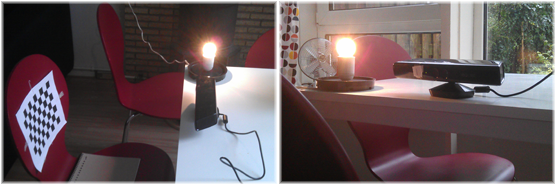
\includegraphics[scale=0.6]{images/calibrating.png}
\caption{Calibrating arrangement}
\label{fig:calibrating}
\end{figure}

The main challenge here is to find a good way to get the image and object points. Thanks to the fact that we \emph{are} able to get the raw infrared image from the Kinect (see section \ref{sec:mod_to_freenect}), we can use OpenCV's automatic chessboard recognition for both cameras. The Kinect's dot pattern however distorts the infrared image. Therefore, the infrared projector should be covered when calibrating (like in figure \ref{fig:calibrating}).  Using this, we find the image points.

Since we know the properties of a checkerboard, we can also derive the object points:
\[
\left[ \begin{array}{ccc}
\left(0, 0, 0\right), & \left(1, 0, 0\right), & ...,\\
\left(0, 1, 0\right), & \left(1, 1, 0\right), & ...,\\
..., & ..., & ...
\end{array}\right]
\]

\begin{figure}[H]
\centering
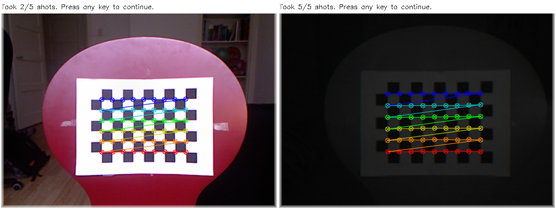
\includegraphics[scale=0.6]{images/chessboard.png}
\caption{Chessboard recognition in both the RGB and IR image}
\label{fig:chessboard}
\end{figure}

As can be seen in figure \ref{fig:chessboard}, the chessboard corners are easily found. From this, the intrinsic matrices will be generated. Now that we know the intrinsic matrices for both cameras, we can start looking for the rotation matrix and translation vector between the coordinate systems of both cameras. In OpenCV, this is done by the function \verb|StereoCalibrate| (see figure \ref{code:stereocalibrate}). 

\begin{figure}[H]
\begin{lstlisting}
StereoCalibrate(objectPoints, imagePoints1, imagePoints2, pointCounts, cameraMatrix1, distCoeffs1, cameraMatrix2, distCoeffs2, imageSize, R, T, E=None, F=None, term_crit=(CV_TERMCRIT_ITER+CV_TERMCRIT_EPS, 30, 1e-6), flags=CV_CALIB_FIX_INTRINSIC)
\end{lstlisting}
\caption{OpenCV stereo calibration function}
\label{code:stereocalibrate}
\end{figure}

Again, you need the object and image points from both cameras. You also need both cameras' intrinsic matrix and distortion coefficients. Just like we need, this function ouputs the rotation matrix and translation vector between the coordinate systems of both cameras. There is some other optional output, but we don't need that here.

\subsubsection{Disclaimer}
Despite all our hard work, we still can't find the right camera matrices nor the correct rotations between the coordinate spaces of both cameras. At first we thought something went wrong at the initialization of the object points, but it turned out this wasn't the problem. Also, the chessboard recognition works fine and finds the right image points. After spending two whole weekends on it, we gave up.

%TODO: reference to http://nicolas.burrus.name/index.php/Research/KinectCalibration
Luckily, this doesn't mean that we are stuck here. While wandering around on the internet, we found the matrices Nicolas Burrus has estimated for his Kinect. Although these matrices will differ slightly from our own, they turned out to give pretty good results (see also section \ref{sec:alignment}). We therefore decided to use these instead of our own.


\subsection{Aligning depth and color images}

\subsubsection{Rectification}
In order to align the depth image with the color image from the Kinect, these images first need to be rectified. Rectification is the process that reprojects image planes so that they reside in
the exact same plane and their epipolar lines become parallel. In OpenCV, you need three functions to rectify an image. The first one is \verb|StereoRectify| (see figure \ref{code:stereorectify}).

\begin{figure}[H]
\begin{lstlisting}
StereoRectify(cameraMatrix1, cameraMatrix2, distCoeffs1, distCoeffs2, imageSize, R, T, R1, R2, P1, P2, Q=NULL, flags=CV_CALIB_ZERO_DISPARITY, alpha=-1, newImageSize=(0, 0))
\end{lstlisting}
\caption{OpenCV stereo rectification function}
\label{code:stereorectify}
\end{figure}

In order to call this function, you need the camera matrices and distortion coefficients as well as the rotation matrix and the translation vector between those cameras. These were derived in the calibration step (see section \ref{sec:stereo_calibrate}). The function finally returns four matrices: R1, R2, P1 and P2. R1 and R2 are the rectification transforms for the first and second camera, respectively. P1 and P2 are the projection matrices in the new rectified coordinate systems. These four matrices can be used in the next step: \verb|InitUndistortRectifyMap| (see figure \ref{code:initrecmap}).

\begin{figure}[H]
\begin{lstlisting}
InitUndistortRectifyMap(cameraMatrix, distCoeffs, R, P, mapx, mapy)
\end{lstlisting}
\caption{OpenCV initialization of the rectification maps}
\label{code:initrecmap}
\end{figure}

As you can see, this function only takes one camera matrix, one set of distortion coefficients, etcetera. This indicates that we have to call this function twice: once for the depth image and once for the color image. The function returns two maps, \verb|mapx| and \verb|mapy|, that map the pixels of an image to the right position in the rectified image. This mapping process is done in the final step of rectification: \verb|Remap| (see figure \ref{code:remap}).

\begin{figure}[H]
\begin{lstlisting}
Remap(src, dst, mapx, mapy, flags=CV_INNER_LINEAR+CV_WARP_FILL_OUTLIERS, fillval=(0, 0, 0, 0)) 
\end{lstlisting}
\caption{OpenCV remap function}
\label{code:remap}
\end{figure}

When we provide this function with a non-rectified image (\verb|src|) and two maps (\verb|mapx| and \verb|mapy|), these maps are applied to the image. The resulting image (\verb|dist|) will now be the rectified image we've been looking for (e.g. figure \ref{fig:rectify}).

\begin{figure}[H]
\centering
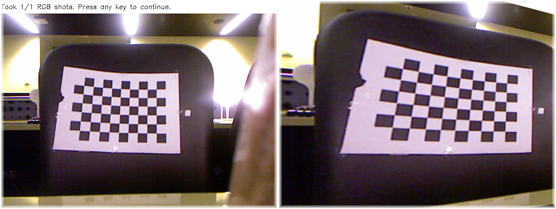
\includegraphics[scale=0.6]{images/rectify.png}
\caption{Raw (left) and rectified (right) color image}
\label{fig:rectify}
\end{figure}


\subsubsection{Alignment}
\label{sec:alignment}

\begin{figure}[H]
\centering
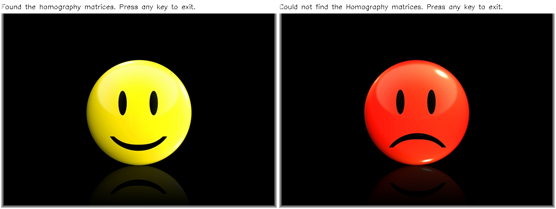
\includegraphics[scale=0.6]{images/homography.png}
\caption{Good and bad result of FindHomography}
\label{fig:homography}
\end{figure}

Now that we've rectified both images, we just have to translate them so that they're completely aligned (i.e., a pixel $\left(x, y\right)$ in the color image is the same pixel at $\left(x, y\right)$ in the depth image). This final translation could be found by just finding one corresponding point in each image, but to minimize distortion, we've decided to, again, use chessboard recognition. Since we still have the images of both the depth and the color camera at calibration time, we can reuse those. After rectifying them, we can create a collection of chessboard corners in the rectified images. Since we use multiple points, we can't use \verb|GetAffineTransform| (max. 3 points) or \verb|GetPerspectiveTransform| (max. 4 points), but we have to use \verb|FindHomography| (see figure \ref{code:findhomography}). As you can see in figure \ref{fig:homography}, this process doesn't always end well. When we use our own derived camera matrices, the process fails, since the rectification matrices are wrong. Otherwise, when we use Nicolas Burrus' matrices, the process ends well. More about this can be found in section \ref{sec:stereo_calibrate}.

\begin{figure}[H]
\begin{lstlisting}
FindHomography(srcPoints, dstPoints, H, method=CV_RANSAC, ransacReprojThreshold=3.0, status=None)
\end{lstlisting}
\caption{OpenCV remap function}
\label{code:findhomography}
\end{figure}

Here, \verb|scrPoints| is the collection of chessboard corners in the rectified depth images, \verb|dstPoints| the collection of chessboard points in the rectified rgb images. The homography matrix (\verb|H|) gives us the final translation between the color and depth images. All we need to do now is apply this translation to the depth image. This can be done by the OpenCV function \verb|WarpPerspective| (see figure \ref{code:warpperspective}).

\begin{figure}[H]
\begin{lstlisting}
WarpPerspective(src, dst, mapMatrix, flags=CV_INNER_LINEAR+CV_WARP_FILL_OUTLIERS, fillval=(0, 0, 0, 0))
\end{lstlisting}
\caption{OpenCV remap function}
\label{code:warpperspective}
\end{figure}

Given a source image (\verb|src|) and a map matrix (\verb|mapMatrix|, we use \verb|H| here), this function gives the resulting image of applying that matrix to the image (\verb|dst|). In figure \ref{fig:aligned}, you can see that the aligned images overlay perfectly.

\begin{figure}[H]
\centering
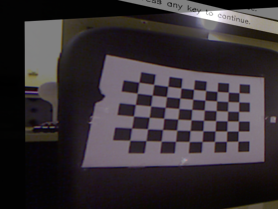
\includegraphics[scale=0.6]{images/aligned.png}
\caption{Overlayed aligned RGB and IR images}
\label{fig:aligned}
\end{figure}


\subsection{Getting the `real' depth}
The Kinect's depth output is not on a linear scale. Therefore, if we want to create a 3D object scanner, we have to convert the depth to a linear scale. Because of the short range of the Kinect, we chose to use centimeters as this scale. We found the following formula:

\begin{lstlisting}
def depth_to_centimeters(d):
    if d < 2047:
        return 12.36 * tan(d / 2842.5 + 1.1863)
    else:
        return -1.0
\end{lstlisting}
%TODO add reference to http://groups.google.com/group/openkinect/browse_thread/thread/31351846fd33c78/e98a94ac605b9f21?lnk=gst&q=stephane#e98a94ac605b9f21
This function was provided by Dr. St\'ephane Magnenat, but was never derived nor proven. A few tests however showed that it is quite a good approximation.

What may seem odd here is the \verb|if d < 2047| statement, but it isn't. The depth value the kinect returns when it cannot find the depth for a certain point (e.g. when the point is too far away) is 2047. Since we don't want this point to be in our 3D space, we remove it.

\subsection{Creating a model}

\subsubsection{The algorithm}

%todo: with "stereo calibrate" do you mean some kinect interface module or our
%own stereo calibration step? I am assuming the latter for now...

Information derived at the stereo\texttt{stereo calibrate} stage will help with
pre-processing the Kinect image streams. We notably obtained: two intrinsic
matrices; two sets of distortion coefficients; two rotation matrices; and two
translation matrices. All these matrices can be used to undistort both images,
so that an object in the depth image is in the same place as an object in the
RGB image. We undistort the images using the \texttt{InitUndistortRectifyMap}
function from OpenCV.

With the two image streams pre-processed, the application proceeds to build the
model. The first step is to determine the ``working field''. This is done with
an A3-size sheet of white paper placed on a flat surface. The corners of the
sheet are colored (in order) green, blue, red and black.

For now, the application requires users to manually determine the orientation of
the working field. The \texttt{create\_model.py} module prompts the user to
click on the pixels in the RGB image corresponding to the coloured corners of
the A3 sheet (see figure \ref{fig:clicking}). Information displayed in the image helps the user to select the points in the correct order.

\begin{figure}[H]
\centering
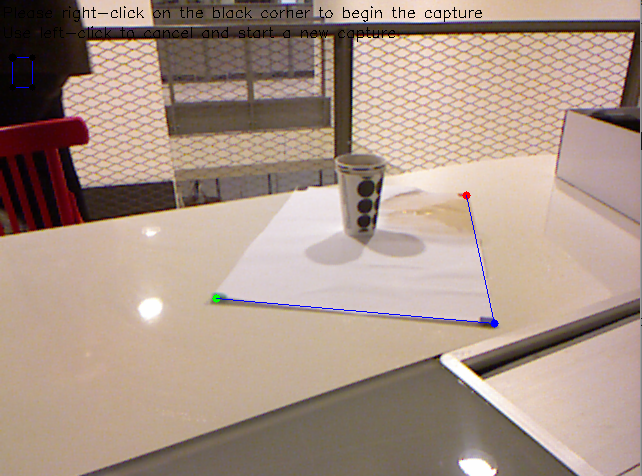
\includegraphics[scale=0.5]{images/clicking.png}
\caption{Clicking on the corners of the working field}
\label{fig:clicking}
\end{figure}

With the help of the $z$ values from the depth image, the selected points'
$(x,y,z)$ coordinates are determined. The code displayed in \ref{code:cube}
derives from this information all 8 points of a ``working cube''.\\

\begin{figure}[H]
\begin{lstlisting}
for i in xrange(4):
    cubic.append(np.array([points[i][0],points[i][1],sqrt(depth[points[i][1]][points[i][0]]]), dtype=float))
    if depth[points[i][1]][points[i][0]] > 2000:
        print "Point no. ", i, " is probably in a blind spot. Please start over."


for i in xrange(4):
    cubic = cubic + [np.cross((cubic[((i + 1) % 4)] - cubic[i]),(cubic[((i + 3) % 4)] - cubic[i]))]
    cubic[i + 4] = cubic[i + 4] / np.linalg.norm(cubic[i + 4])
    cubic[i + 4] = (cubic[i + 4] * height) + cubic[i]
\end{lstlisting}
\caption{Algorithm to create a 3 dimensional cube}
\label{code:cube}
\end{figure}

Since the working cube coordinates derived in this way are relatively
inaccurate, they are only used to overlay the cube's wireframe on the rgb and
depth images for the user's benefit. This enables the user to determine whether
they have correctly identified the working field to the application, and then to
proceed or start over as necessary.

All the ingredients to begin obtaining points for our 3d representation are now
in place:
\begin{itemize}

\item Four user-selected working field points.

\item A calibrated numpy array containing the whole RGB image as it was at the
moment of the first first click;

\item A calibrated numpy array containing the whole depth image, also from the
moment of the first click.

\end{itemize}

For each point in the image, the application needs to determine the
corresponding point in the object space. The object space was represented to the
user with the ``working cube'' wireframe. Now the application derives the axes
of the object coordinate system from the predetermined order in which the user
selected the coloured working plane corners. The following convention applies:
\begin{itemize}

\item The origin is in the corner of the cube ``above'' the green corner of the
working field.

\item The x axis runs through the origin and the working cube corner ``above'' the
working field's blue corner.

\item The y axis runs through the origin and the working field's green corner.

\item The z axis runs through the origin and the point ``above'' the working
field's black corner

\end{itemize}

The result is visualized in figure \ref{fig:axis}.

\begin{figure}[H]
\centering
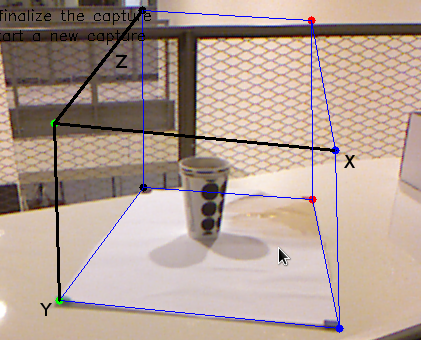
\includegraphics[scale=0.5]{images/axis.png}
\caption{Calculated cube, with axis}
\label{fig:axis}
\end{figure}

The cube's dimensions are then normalised to $100$ respectively in the $x$ and
$y$ directions, and $141$ for the $z$ direction. The last dimension is the value
of $100\sqrt 2$, which in turn is the length to width ratio of an A3 sheet.
The manually selected points can now be translated to object space coordinates
as follows:
$$
\vec{green} = \left[ \begin{array}{ccc} 
0\\
100\\
0  \end{array} \right], \quad
\vec{blue} = \left[ \begin{array}{ccc} 
100\\
100\\
0  \end{array} \right], \quad
\vec{red} = \left[ \begin{array}{ccc} 
100\\
100\\
141  \end{array} \right], \quad
\vec{black} = \left[ \begin{array}{ccc} 
0\\
100\\
141  \end{array} \right].
$$
The points in object space are last information necessary to use the
\texttt{FindExtrinsic\-CameraParams2} function from OpenCV. Because the image is
undistorted during pre-processing, the identity matrix serves as the intrinsic
matrix, and \texttt{NULL} is passed as the distortion parameter. The function
returns a rotation matrix vector and a translation vector. A rotation matrix is
derived from the rotation vector using the \texttt{rodrigues2} function in
OpenCV. Then, the extrinsic matrix is derived from the translation vector. 

The resulting information can be inserted in the following equation:
\begin{equation}\label{eq:pipeline}
s \left[ \begin{array}{ccc} 
u\\
v\\
1 \end{array} \right] = 
\left[ \begin{array}{ccc} 
f_{x} & 0 & c_{x}\\
0 & f_{y} & c_{y}\\
0 & 0 & 1 \end{array} \right] 
\left[ \begin{array}{cccc} 
r_{11} & r_{12} & r_{13} & t_{1}\\
r_{21} & r_{22} & r_{23} & t_{2}\\
r_{31} & r_{32} & r_{33} & t_{3} \end{array} \right] 
\left[ \begin{array}{ccc} 
x\\
y\\
z\\
1  \end{array} \right] 
.
\end{equation}
In this equation,
$$
\left[ \begin{array}{ccc} 
u\\
v\\
1 \end{array} \right]
$$
are the image coordinates,
$$
\left[ \begin{array}{ccc} 
x\\
y\\
z\\
1  \end{array} \right] 
$$
are the coordinates in object space,
$$
\left[ \begin{array}{ccc} 
f_{x} & 0 & c_{x}\\
0 & f_{y} & x_{y}\\
0 & 0 & 1 \end{array} \right]
$$
is the intrinsic matrix (identity) and
$$
\left[ \begin{array}{cccc} 
r_{11} & r_{12} & r_{13} & t_{1}\\
r_{21} & r_{22} & r_{23} & t_{2}\\
r_{31} & r_{32} & r_{33} & t_{3}
\end{array} \right]
$$
is the extrinsic matrix \cite{OPENCV}.

At this point, we can take the depth value at every point in the depth image for
the $s$ value in the above equation. So $s = d(u,v)$. At this point, we know
the vector $$
\left[ \begin{array}{ccc} 
u s\\
v s\\
s \end{array} \right].
$$ for every point in the depth image and for every point in the rgb image. We 
can now translate it to $(x,y,z)$ coordinates in our object space with the 
following equation:
$$
\left[ \begin{array}{c} 
x\\
y\\
z\end{array} \right] 
=
\left[ \begin{array}{ccc} 
r_{11} & r_{12} & r_{13}\\
r_{21} & r_{22} & r_{23}\\
r_{31} & r_{32} & r_{33}
\end{array} \right]^{-1}
\left[ \begin{array}{c} 
u s\\
v s\\
s \end{array} \right]
-
\left[ \begin{array}{c} 
t_{1}\\
t_{2}\\
t_{3}
\end{array} \right]
$$
We pass all (x,y,z) coordinates to the point cloud viewer, including 
the corresponding color value. \\
\\
As you might have noticed, the intrinsic matrix isn't used in the last equation.
This is because (as we mentioned earlier) the images were already undistorted
and rectified.

\subsubsection{Defects and todo}

Defects (at the time of writing):

\begin{itemize}

\item Something goes wrong in the FindExtrinsicCameraParams2, it returns NaN for the translation vector.

\item We still work with distorted images, since the stereo calibration wasn't done.

\item We don't know if the cubicle size is correct.

\item We haven't implemented anything after we needed after FindExtrinsicCameraParams2 because it doesn't work

\end{itemize}

Todo: 

\begin{itemize}

\item Undistort and rectify the images%todo

\item Find a replacement for FindExtrinsicCameraParams2%todo

\item Apply the extrinsic matrix to all object points and check if values of those points are between the depth boundaries.%todo

\item Send points to the point cloud viewer%todo

\item Color the points using the rgb image%todo

\item Auto detect the corners of our "working field"%todo

\end{itemize}

\subsection{Point Cloud Viewer}

The point cloud viewer was developed after examining various possible
bases, such as: PCL(see pointclouds.org, A very large production-class project for
anything to do with point clouds), PyGame and Visual. Visual is also know
as VPython.

For a very short period of time we tried using the mpl\_toolkit provided
by matplotlib, but as it has no support for OpenGL it isn't very suited
for rendering a large amount of points in 3D.

The PCL library was of course
very tempting, but very soon it became apparent this was way too much horse
power for our needs. What we needed was a simple interface that allowed viewing
of point clouds, rotating, moving and zooming them with mouse and keyboard
controls.

PyGame allows for very easy initialisation of OpenGL using SDL and can therefore
easily handle point clouds using most of today's graphics hardware. But it still
did not provide an easy way of controlling the camera. Rotation would require
using some sort of mathematical library implementing quaternion spherical rotation.

Enter VPython, a package attempting to implement a simple 3D programming
language on top of Python and allowing interactive terminal control of the
3D scene. VPython officially is composed of: Python (of course), IDLE the
interactive Python programming environment and the visual module. When we
discoverd the visual module used OpenGL, offers mouse orientation
controls by default, and to top it off uses NumPy for all its data manipulation
our course of action became very clear. Since the Kinect library provides its
data in NumPy arrays, after simple manipulation the point clouds can be fed into
visual with the simple command "points".

Currently the point cloud viewer does not support realtime capture, but capture
is done quickly and easily using the 'c' key.

The low-level interface includes the option for depth smoothing.

\subsection{Combining it all}

% in para below: "from files" = the matrices or the images?

The \texttt{Kinect.py} offers a user interface to the application. The file can
be executed using command line arguments to load matrices for undistoring and
rectifying the images from files. Once executed, the \texttt{Kinect.py} module
offers the user a menu. The first menu item offers a calibration process in case
this has not yet been performed.  Via the second menu choice the user can start
to build a 3d model. This opens: a point cloud viewer; an ``rgb'' screen that
displays images from the rgb camera; and a ``depth'' screen that displays depth
camera images. Whenever the user triggers an image capture, all points are sent
to the point cloud viewer. Pressing \texttt{esc} closes all windows and returns
the user to the menu.
